%%%%%%%%%%%%%%%%%%%%%%%%%%%%%%%%%%%%%%%%%
% University/School Laboratory Report
% LaTeX Template
% Version 3.1 (25/3/14)
%
% This template has been downloaded from:
% http://www.LaTeXTemplates.com
%
% Original author:
% Linux and Unix Users Group at Virginia Tech Wiki
% (https://vtluug.org/wiki/Example_LaTeX_chem_lab_report)
%
% License:
% CC BY-NC-SA 3.0 (http://creativecommons.org/licenses/by-nc-sa/3.0/)
%
%%%%%%%%%%%%%%%%%%%%%%%%%%%%%%%%%%%%%%%%%

%----------------------------------------------------------------------------------------
%	PACKAGES AND DOCUMENT CONFIGURATIONS
%----------------------------------------------------------------------------------------

\documentclass{article}

\usepackage{float} % Required for images to be placed inline
\usepackage[version=3]{mhchem} % Package for chemical equation typesetting
\usepackage{siunitx} % Provides the \SI{}{} and \si{} command for typesetting SI units
\usepackage{graphicx} % Required for the inclusion of images
\usepackage{natbib} % Required to change bibliography style to APA
\usepackage{amsmath} % Required for some math elements

\setlength\parindent{0pt} % Removes all indentation from paragraphs

\renewcommand{\labelenumi}{\alph{enumi}.} % Make numbering in the enumerate environment by letter rather than number (e.g. section 6)

%\usepackage{times} % Uncomment to use the Times New Roman font

%----------------------------------------------------------------------------------------
%	DOCUMENT INFORMATION
%----------------------------------------------------------------------------------------

\title{Electric Field and Potential\\ PHY-222-AC01} % Title

\author{Jasper \textsc{Runco}} % Author name

\date{\today} % Date for the report

\begin{document}

\maketitle % Insert the title, author and date


%----------------------------------------------------------------------------------------
%	SECTION 1
%----------------------------------------------------------------------------------------

\section{Theory}

\paragraph{Electric Field of the Point Charge:}

In the previous lab, the interaction of charged objects at a distance was studied and we concluded
that the phenomenon of an electric force pair exists along the path connecting the charged objects
with opposite direction depending on parity of the charge carriers (opposites attract). The magnitude
of the electric force is defined by Coulomb's law.
\newline

When studying the electric force generated by a given
localized charge, it is very useful to construct a vector field at all posible points in space around
the localized charge. The fact that our localized charge may be continuous distributions of charge
across surfaces or volumes is problematic. The resulting vector field should not be ambiguous. To avoid
this wherever possible, we can use Coulomb's equation to derive an equation that generates a vector field
around a point charge, a hypothetical $e_{-}$ or $e_{+}$, and use calculus to extrapolate this vector
field to the entire charged region
\newline

Given the similarities between Coulomb's law and Newton's law of gravitation, calling this calculation
an electric field is likely a poor choice of wording. We should be careful not to exagerate what this
"electric field" describes. We have already seen that Newton's gravity gave rise to relativity, in which
gravity went from being a force to a field that affects the geometric proporties of space-time. A vector
field calculation gives a good insight for possible electric forces, but these are labels, not nesecarily
properties.



%----------------------------------------------------------------------------------------
%	SECTION 2
%----------------------------------------------------------------------------------------
\section{Objectives}


% If you have more than one objective, uncomment the below:
\begin{description}
	\item[First Objective] \hfill \\
		Verify the formula for the electric field of the point charge.
	\item[Second Objective] \hfill \\
		Explore the electric field lines of various charge configurations and the
		superposition principle.
	\item[Third Objective] \hfill \\
		Explore the relationship between the electric field and electric potential.
\end{description}


%----------------------------------------------------------------------------------------
%	SECTION 3
%----------------------------------------------------------------------------------------

\section{Experimental Data}

\subsection{Part I}%
\label{sub:part_one}

\subsubsection{Qualitative Data}%
\label{ssub:qualitative_data}


\begin{figure}[H]
	\begin{center}
		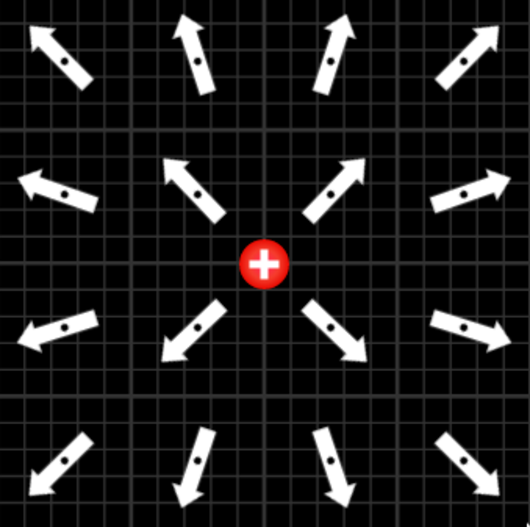
\includegraphics[width=0.65\textwidth]{part-1-simulation.pdf} % Include the image placeholder.png
		\caption{Part 1.1 Simulation}
	\end{center}
\end{figure}

\subsubsection{Quantitative Data}%
\label{ssub:quantitative_data}

\begin{figure}[H]
	\begin{center}
		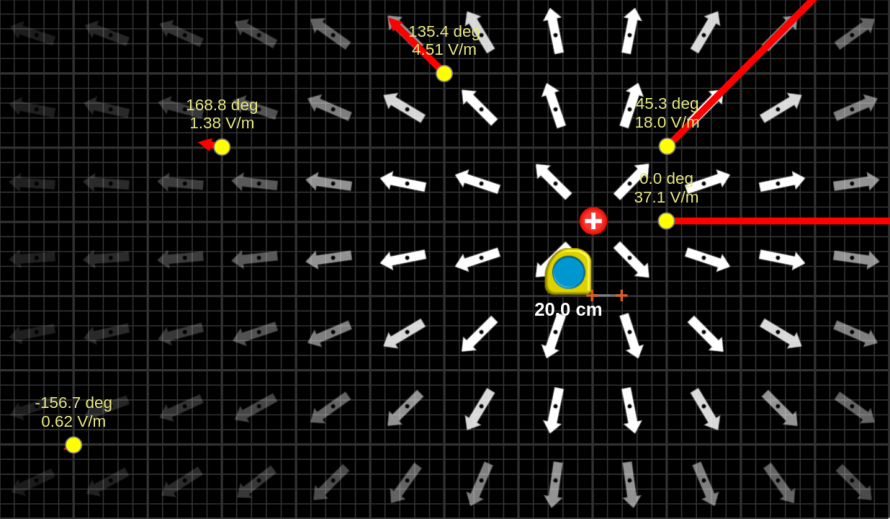
\includegraphics[width=0.65\textwidth]{part-2-simulation.pdf} % Include the image placeholder.png
		\caption{Part 1.2 Simulation}
	\end{center}
\end{figure}

\begin{table}[htpb]
	\centering
	\caption{Part 1.2}
	\label{tab:label}
	\begin{tabular}{| l | l | l | l | l | l | l |}
	\hline
	\tiny Sensor \# & \tiny $x$ (cm) & \tiny$y$ (cm) & \tiny$r = \sqrt{x^2+y^2} $ (cm) & \tiny$\theta = \arctan \frac{y}{x}$ (rad) & \tiny$\left| \overline{E} \right| $ (V/m) & \tiny Electric Field angle (degrees)\\
	\hline
	1  & $50.0$ & $0.0$ & $50.0$ & 0.0 & 37.1 & 0.0\\
	\hline
	2  & $50.0$ & $50.0$ & $70.7$& $0.785$ & 18.0 & 45.3\\
	\hline
	3  & $-100.0$ & $100.0$ & $141.4$ & $2.356$ & 4.51 & 135.4\\
	\hline
	4  & $-250.0$ & $ 50.0$ & $255.0$ & $2.94$ & 1.38 & 168.8\\
	\hline
	5  & $-350.0$ &  $-150.0$ & $380.8$ & $-2.737$ & 0.62 & -156.7\\
	\hline
	\end{tabular}
\end{table}

\subsection{Part II}%
\label{sub:part_two}

\begin{figure}[H]
	\begin{center}
		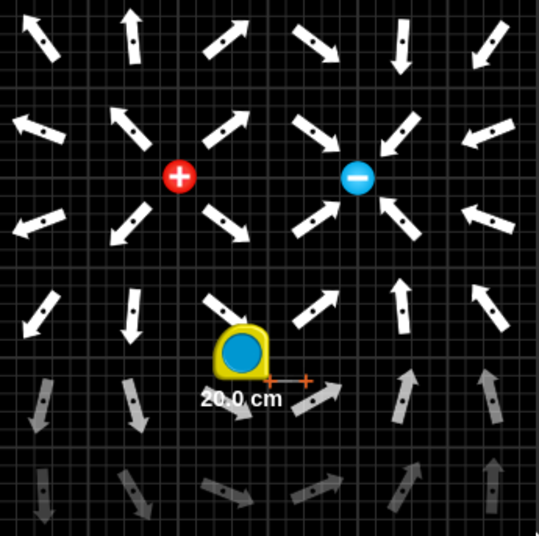
\includegraphics[width=0.65\textwidth]{simulation-1.2} % Include the image placeholder.png
		\caption{Part 2.1-2.3 Simulation}
	\end{center}
\end{figure}

\begin{figure}[H]
	\begin{center}
		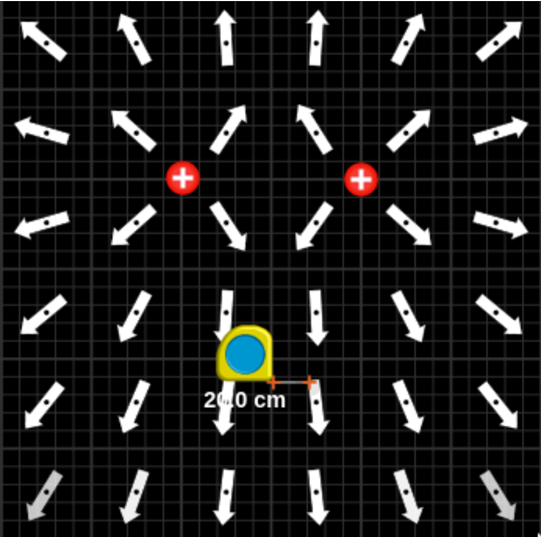
\includegraphics[width=0.65\textwidth]{part-2.4-2.5-simulation} % Include the image placeholder.png
		\caption{part 2.4-2.5 simulation}
	\end{center}
\end{figure}

\begin{figure}[H]
	\begin{center}
		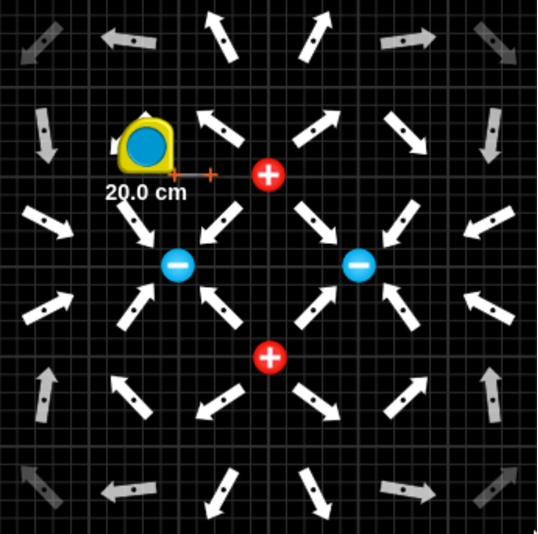
\includegraphics[width=0.65\textwidth]{part-2.5-simulation} % Include the image placeholder.png
		\caption{part 2.6 simulation}
	\end{center}
\end{figure}

\begin{figure}[H]
	\begin{center}
		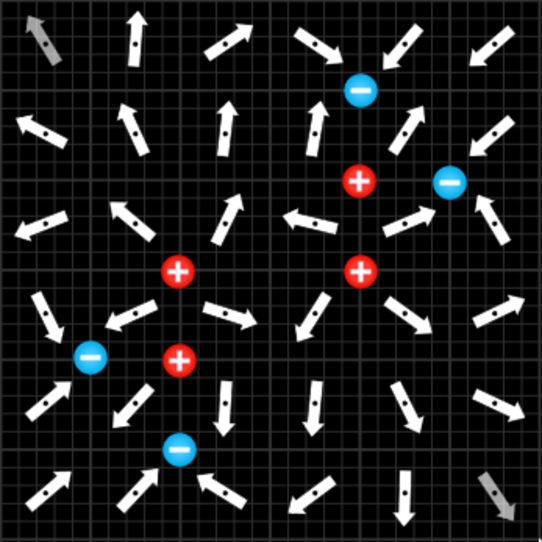
\includegraphics[width=0.65\textwidth]{part-2.7-simulation} % Include the image placeholder.png
		\caption{part 2.7 simulation}
	\end{center}
\end{figure}

\subsection{Part III}%
\label{sub:part_3}

\begin{figure}[H]
	\begin{center}
		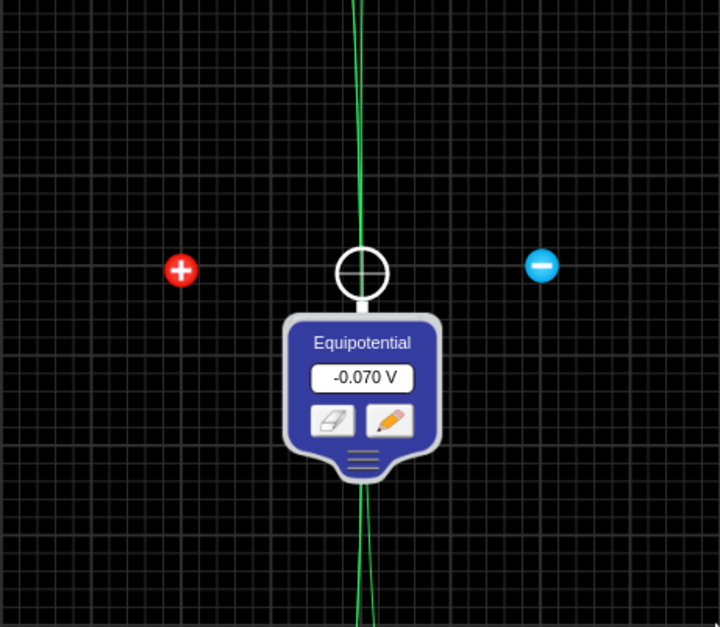
\includegraphics[width=0.65\textwidth]{part-3.2-simulation} % Include the image placeholder.png
		\caption{part 3.2 simulation}
	\end{center}
\end{figure}

\begin{figure}[H]
	\begin{center}
		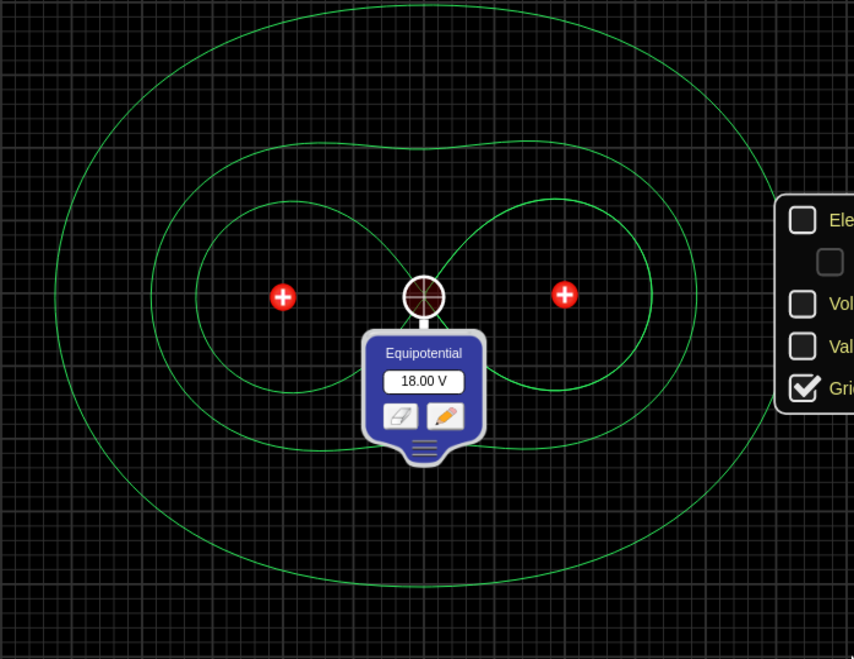
\includegraphics[width=0.65\textwidth]{part-3.3-simulation} % Include the image placeholder.png
		\caption{part 3.3 simulation}
	\end{center}
\end{figure}

\subsection{Part IV}%
\label{sub:part_4}

\begin{figure}[H]
	\begin{center}
		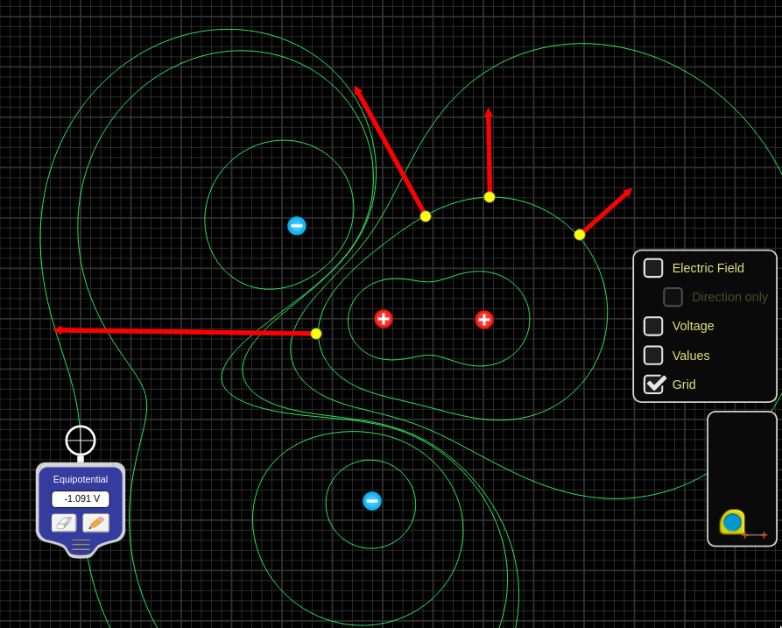
\includegraphics[width=0.65\textwidth]{part-4-simulation} % Include the image placeholder.png
		\caption{part 4.1 simulation}
	\end{center}
\end{figure}

\begin{figure}[H]
	\begin{center}
		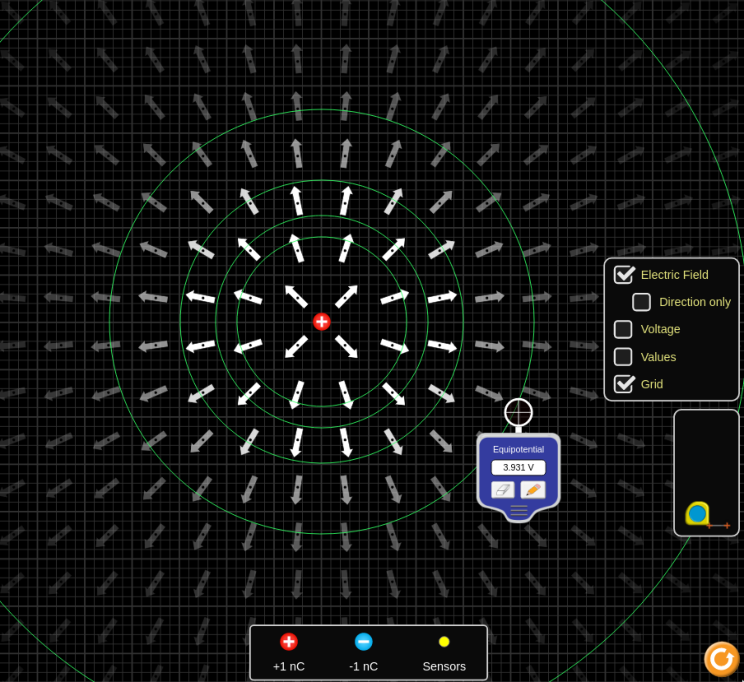
\includegraphics[width=0.65\textwidth]{part-4.2-simulation} % Include the image placeholder.png
		\caption{part 4.2 simulation}
	\end{center}
\end{figure}




%----------------------------------------------------------------------------------------
%	SECTION 4
%----------------------------------------------------------------------------------------

\section{Data Analysis}

\subsection{Part I}%
\label{sub:part_one}

\subsubsection{\textbf{Can the arrows that the program uses to visualize the electric field be called field lines? How are they similar and different from the field lines?}}
\label{ssub:}

The arrows could be used to visualize the electric field lines, but they are not lines.
Like electric field lines, the arrows indicate the direction and strength of the electric field.
The lines indicate the relative strength of the field in a different way. The opacity of the arrows
describes the field strength while field lines show field strength with their proximity to adjacent field lines.

\subsubsection{Section 2}%
\label{ssub:part_2}

a) The angle of the position vector of the test charges is equal to the angle of the electric field
in every test charge in this experiment. This suggests a theory that the electric field is directed radially.
To prove that the electric field of the point charge is radial by
statistical proof would warrant more data.

b) See Table 2. The fourth column, $\overline{E} \times  r^2$ (Vm), does show that the magnitude of
the electric field is inversely proportional to the distance squared because their product is constant.
Sensor 1 is an outlier, and the median is sensor 2 at 9.00 Vm. Sensor 2 will be used to calculate k.

\begin{align*}
\left| \overline{E} \right| &=  \frac{kq}{r^2} \implies \\
k &= \frac{\left| \overline{E} \right| r^2}{q} \\
k &= \frac{18.0 \frac{V}{m} \cdot (70.7 cm)^2}{1nC} \\
k &= \frac{18.0 \frac{N}{C} \cdot (0.707 m)^2}{10^{-9}C} \\
k &= \boxed{9.00 \times 10^{9}\frac{Nm^2}{C^2} }\\
\end{align*}


\begin{table}[htpb]
	\centering
	\caption{Part 1.2}
	\label{tab:label}
	\begin{tabular}{| l | l | l | l |}
	\hline
	\tiny Sensor \# &  \tiny$r = \sqrt{x^2+y^2} $ (cm) & \tiny$\left| \overline{E} \right| $ (V/m) & \tiny $\left| \overline{E} \right| \times r^2$ (Vm)\\
	\hline
	1  &   $50.0$ &  37.1 & 9.27\\
	\hline
	2  &   $70.7$&  18.0 & 9.00\\
	\hline
	3  &   $141.4$  & 4.51 & 9.02\\
	\hline
	4  &   $255.0$ & 1.38 & 8.97\\
	\hline
	5  &  $380.8$  & 0.62 & 8.99\\
	\hline
	\end{tabular}
\end{table}


\textbf{Question:} Using a negative point charge, the electric field angle measurements
would be anti-parallel to the values for a positive point charge ($\pm \pi$ rad). All other
values would be the same.


\subsection{Part II}%
\label{sub:part_2}

\subsubsection{Section 2: Field Line Description}%
\label{ssub:field_line_description}

\begin{itemize}
	\item On the horizontal axis to the right of the dipole, the field is pointing left
		because the charges superimpose in line, negating each other but the negative charge has a greater effect because it is closer.
	\item On the horizontal axis between charges, the field is in the positive-x direction
		because the charges superimpose in line but from opposite directions, creating a cumulative effect.
	\item On the horizontal axis to the left of the dipole, the field is pointing left
		because the charges superimpose in line, negating each other but the positive charge has a greater effect because it is closer.
	\item Along the vertical bisector above the dipole, the field is to the right because the vertical components of the superimposed fields are equal in magnitude
		and opposite in direction and the horizontal components of the two charges combine in the positive x direction.
		The field strength diminishes farther in the positive-y direction.
	\item Along the vertical bisector below the dipole, the field behaves the same as above the dipole for the
		same reasons, except the field strength diminishes farther in the negative-y direction.
\end{itemize}

\subsubsection{Section 3: Is there a location where the electric field is exactly zero?}%
\label{ssub:is_there_a_location_where_the_electric_field_is_exactly_zero_}

In the case of an electric dipole, at no position do the electric fields of the two charges cancel.

\subsubsection{Section 4: Field Line Description}%
\label{ssub:field_line_description}

\begin{itemize}
	\item On the horizontal axis to the right of the dipole, the field is pointing right
		because the charges superimpose in line, reinforcing each other.
	\item On the horizontal axis between charges, the field points away from whichever charge
		is closer because the charges superimpose in line but in opposite directions. Field strength increases
		closer to either positive charge.
	\item On the horizontal axis to the left of the dipole, the field is pointing left
		because the charges superimpose in line, reinforcing each other.
	\item Along the vertical bisector above the dipole, the field in the positive-y direction because the horizontal components of the superimposed fields are equal in magnitude
		and opposite in direction and the vertical components of the two charges combine in the positive y direction.
		Field strength diminishes farther from the charges.
	\item Along the vertical bisector below the dipole, the field behaves the same as above the dipole for the
		same reasons, except field strength diminishes farther in the negative-y direction.
\end{itemize}

\subsubsection{Section 5: Is there a location where the electric field is exactly zero?}%
\label{ssub:is_there_a_location_where_the_electric_field_is_exactly_zero_}
Yes, the only location where the field strength is zero is along the x-axis
at the bisector of the two charges.

\subsubsection{Section 6: See Figure 5}%
\label{ssub:section_6_see_figure_5}

\subsubsection{Section 7: See Figure 6}%
\label{ssub:section_6_see_figure_5}


\subsection{Part III}%
\label{sub:part_iii}

See Figure 7 and Figure 8

Based on these observations, electric field superposition with opposite charges behaves like the potential
superposition with like charges. In other words, a pair of positive charges or a pair of negative charges
will have a cumulative effect of electrical potential, but a diminishing effect on electric field.


\subsection{Part IV}%
\label{sub:part_iv}

\subsection{Section 1}%
\label{sub:section_1}

See Figure 9. The voltage sensor reads the same at every point on these lines,
indicating that these are equipotential lines over this charged surface.
The electric field at every point on the line is always perpendicular to the line itself. The field magnitude
increases with proximity to the point charges, where the exhibit closer proximity to
each other.


\subsection{Section 2}%
\label{sub:section_2}

See Figure 10. The lines that are closer to each other occur in the regions
where the strength of the electric field is greater.



\section{Conclusion}%
\label{sec:conclusion}

These experiments demonstrate several relationships between electric field lines
and electrical potential. First, the two are mutually perpendicular.
Second, movement in the direction of an electric field results in
a decrease in the electrical potential. Because work has an inverse relationship
with potential energy, it is comparable to say work is done by the electric field
to a particle that moves through the electric field. Finally, if a field is mapped
with equipotential lines where the difference in potential between neighboring lines
is the same, then the field strength is going to be greater in regions where the
equipotential lines are closer. In a two-dimensional field, the field is like a
topographical map with the equipotential lines being elevation and the gradient being
field strength.







%----------------------------------------------------------------------------------------
%	SECTION 5
%----------------------------------------------------------------------------------------


%----------------------------------------------------------------------------------------
%	SECTION 6
%----------------------------------------------------------------------------------------

\section{Discussion of Experimental Uncertainty}

The is a virtual experiment and so there is no source of uncertainty other than
the precision of the programs calculations.

\end{document}
